\section{Background and Related Work}
\label{sec:background}
% subsections are \subsection{title}
%% subssubsections are \subsubsection{title}
%% numbering will work automatically

\subsection{Distributional Hypothesis}

The Distributional Hypothesis is the theory that drives the current and leading models for detecting LSC. The rationale being that “there is a correlation between distributional similarity and meaning similarity, which allows us to utilize the former in order to estimate the latter”—in simpler and more familiar terms, “words which are similar in meaning occur in similar contexts” \citep{sahlgren2008distributional}. The distributional methodology presented in \citet{harris1970distributional} is built on structuralist theory. A structuralist approach to language focuses on the general construction of a language system rather than the idiolectal use of language. According to \citet{sahlgren2008distributional}, \citet{saussure1916} identifies the functional differences of linguistic meaning into syntagmatic and paradigmatic relations. Syntagmatic relations involve the syntactic positioning or sequence of words. The combination and order of linguistic entities form a syntagmatic relationship that then creates meaning. Paradigmatic relations exist between words that appear in the same context but do not co-occur. Given these characteristics, linguistic entities that have a paradigmatic relationship should be interchangeable within the same context or sentence. For example, the sequence of words in the sentence ``I am writing my thesis right now" together form one meaning thus having a syntagmatic relationship. If the word `thesis' is replaced in the sentence, forming ``I am writing my book right now", `thesis' and `book' share a paradigmatic relationship. \citet{sahlgren2008distributional} offers the refined Distributional Hypothesis as, “A distributional model accumulated from co-occurrence information contains syntagmatic relations between words, while a distributional model accumulated from information about shared neighbors contains paradigmatic relations between words.” With this in mind, models with a larger context window are more likely to detect or learn paradigmatic relations. Depending on the manipulation of specific model hyperparameters, certain relations will be learned. 


\subsection{Lexical Semantic Change (LSC)}

LSC detection through computational methods still face many challenges today. \citet{hengchen2021challenges} have identified two approaches in the computational field of LSC—treating a word as an entity and determining semantic change based on its dominant sense and treating each word’s sense as a separate entity. Both approaches however, mostly capture contextual similarity between lexical items while the different levels of meaning\footnote{Referring to \citet{blank1997prinzipien}'s three levels of meaning: language-specific semantic, language-specific lexical, and language-external knowledge. This theory aims to discern the ``levels of word meaning based on which type of knowledge a word can trigger in a human" \citep{hengchen2021challenges}. \citet{blank1997prinzipien}'s theory is not the only theory that attempts to categorise word meaning in levels. However, it is the prevailing theory and foundation in LSC literature.} are seldom distinguished \citep{hengchen2021challenges}. There are three different methods to model the meaning of a word computationally: each word in the vocabulary and all of its semantic information will have one representation (e.g., type embeddings), each word being split into different semantic areas resulting in representations that approximate a word’s senses (e.g., topic modelling), and each word having a representation for every time it is used in a sentence (e.g., contextual embeddings). Each method can be successful when applied appropriately in different tasks and what kind of LSC problem is being solved. It is also important to note that not all approaches are able to model or differentiate the different senses a word could possess. In addition to the word sense limitations these representations have, count representations have also been proven to introduce an inherent dependence on word frequency—resulting in random noise in the models \citep{dubossarsky-etal-2017-outta}. By comparing different corpora with each other, original and shuffled, \citet{dubossarsky-etal-2017-outta} demonstrate that there is a strong correlation between the change scores of words and their frequencies. 

Once words have been created into representations, there are also different measures that can be used when comparing word representations between two time periods (e.g. cosine distance, Euclidean distance, Jensen-Shannon divergence, etc.). With these calculations, there are usually two ways to evaluate large datasets and tasks involving the detection of LSC—through binary LSC (i.e. has a word changed or not) or through graded LSC (i.e. to what degree has a word changed) \citep{schlectwegschulte2020}. Although these approaches present a systematic way of evaluating the current models of meaning being created, the question of what kind of change in meaning a word has undergone remains unanswered.

Corpora and datasets used in the field of LSC are largely in English. However, to assume that semantic change occurs and progresses in identical ways across other languages is extremely incorrect. As stated by \citet{bender_2020}, the advancements in NLP rely on the existence of language resources and English is neither synonymous with nor representative of “Natural Language”. English, as a high-resource language, naturally results in more research findings and published works. The field of LSC is no different. Apart from a handful of corpora in different languages (\citet{diacrita_evalita2020} for Italian, \citet{rodina-kutuzov-2020-rusemshift} and \citet{rushifteval2021} for Russian, and \citet{schlechtweg-etal-2020-semeval} for German, Latin, and Swedish), most research in LSC is conducted on the English language. In order to study semantic change effectively and successfully, the variation that already exists between languages must be considered. The creation of resources for languages other than English is crucial to the development of LSC, and in turn, NLP.   


\subsubsection{Laws of Semantic Change}

The laws of semantic change are not as developed as other established laws in linguistics (e.g., laws of sound change) and the theories supporting these laws have not been developed extensively \citep{Xu2015ACE}. \citet{Xu2015ACE} is an example of a study where two opposing laws of semantic change are examined and evaluated using computational methods and large historical corpora. The law of differentiation suggests that words that are near-synonyms have a tendency to diverge or differentiate in meaning as time progresses while the law of parallel change states that words that have related meanings will change in meaning in the same way (\citet{breal1897essai} and \citet{stern-1921} respectively). \citet{Xu2015ACE} show that the law of parallel change is more prevalent than the law of differentiation in the corpora they have examined. Continued research of semantic change through computational methods allows theories to be confirmed, disproved, or improved upon. 

Extending \citet{hamilton-etal-2016-diachronic}’s proposed method of formulating statistical laws of semantic change through distributional methods in one language, \citet{uban-etal-2019-studying} examine the same laws cross-lingually by calculating the semantic distance of cognate words in numerous languages. Cognates are words in languages from the same language family that share a proto-word. After differentiating cognates and false friends within the corpora, it is shown that “the frequency and polysemy of cognates positively correlate with their cross-lingual semantic shift” \citep{uban-etal-2019-studying}. Conversely, \citet{dubossarsky-etal-2017-outta} disprove the persisting and strong effects of both the Law of Conformity and the Law of Innovation presented in \citet{hamilton-etal-2016-diachronic}. By creating a genuine and a controlled condition, \citet{dubossarsky-etal-2017-outta} observed that the effect of both laws are either not as strong as the research community claims or not existent at all.

%\cmtKV[inline]{REREAD THIS}

%\cmtKV[inline]{unsure how to connect this to this section, but i remember us discussing that this should be brought up}
%\cmtSH[inline]{This was brought up when we discussed that you, unlike the majority of the work before you, looked at different POS-tags. While you do not, in your thesis, investigate whether verbs change more than nouns or whether verbs change more often than nouns or ... etc., you go beyond the pure abstract concept of ``a word is a word" and look at different features. I thought it would be interesting to reflect on that -- you challenge, following a few others, the current status quo}

Although most studies in language change examine semantic change through individual words, there have been some developments in classifying words and examining if there are any similarities in behaviour when undergoing semantic change. After categorising words by their word classes, \citet{dubossarsky2018semantic} found that there is a correlation between word class (i.e. POS-tag) and rate of change in the English language. Verbs change more than nouns and adjectives due to the Verb Mutability Effect which compares the semantic and formal properties of nouns and verbs. While this thesis does not aim to prove or disprove whether these findings are true for the languages being investigated, the target words for the task will be categorised by POS-tags and the models will be tested on these sub-word lists as well. In addition to finding the best overall model for detecting LSC, finding models that perform well detecting semantic change in specific POS-tags could prove very useful for future LSC tasks. 


\subsection{Algorithms}

The two main algorithms used to create word vector representations in this thesis, Word2Vec and FastText, are introduced below. Both type embeddings, Word2Vec and FastText share similar approaches but consider different aspects of language. This form of type embedding was chosen over contextual embeddings since it has shown more promising results in LSC tasks \citep{schlechtweg-etal-2020-semeval}. Recent work on LSC has also shown that both BERT and ELMo do not compete with models trained on Word2Vec and FastText (\citet{schlechtweg-etal-2020-semeval, kaiser-diacrita2020,laicher-2020, uiouva-kutuzovsemeval2020}). The algorithms Word2Vec and FastText will be introduced below. 

%\cmtSH[inline]{Yes I believe a short intro can fit nicely. It will allow you to write a few words about vector space, about how those ``predicting vectors" are ``better" than the count vectors IN NLP IN GENERAL (https://aclanthology.org/P14-1023/ !), and hammer the nail on the fact that until VERY recently the type embeddings were the stars of LSC. Titles of papers such as ``OP-IMS@ DIACR-Ita: Back to the Roots: SGNS+ OP+ CD still rocks Semantic Change Detection" (Kaiser et al 2020) and ``CL-IMS@ DIACR-Ita: Volente o Nolente: BERT does not outperform SGNS on Semantic Change Detection" (Laicher et al 2020) could be mentioned here for example, as a strong reminder of your motivation of using those algos and not BERT.} 

\subsubsection{Word2Vec}
\citet{mikolov2013efficient} proposed two new architectures that use simpler neural networks to learn distributed representations of words while minimizing computational complexity. This resulted in the widely used Word2Vec algorithm that consists of two different model architectures—Continuous Bag-of-Words (CBOW) and Continuous Skip-gram. Both algorithms use a word’s contextual environment (i.e. its surrounding words or context words) to create its semantic representation, in this case, an embedding. The number of neighbouring words before and after (i.e. window size) for training examples is a hyperparameter that can be changed. The three main components of the Word2Vec architecture are a vocabulary builder, a context builder, and a neural network with two layers. The first component’s input is raw text from a corpus and it creates a vocabulary containing all of the unique words and the number of occurrences for each word within the corpus. The context builder then uses the output of the vocabulary builder to create word pairings before and after the target word depending on the context size. Finally, the neural network consists of an input layer, a hidden layer, and an output layer which is then put through a softmax classifier to convert the output into probabilities. Since the vector’s shape is the size of the vocabulary, the final vector contains the probability of each word appearing beside the target word. 

In the CBOW model, the target word is predicted through the distributional representations of the context words. However, in the Skip-gram model, the input and output are the inverse of CBOW—the context words are predicted using the target word.  Skip-gram performs well when used on smaller datasets and have better representations of less frequent words while CBOW models train faster and have better representations of more frequent words \citep{mikolov2013efficient}. Both algorithms were evaluated through performing basic algebraic equations using the vector representations of words to substantiate the models’ ability to identify both semantic and syntactic relationships between words. This seminal paper is now a building block for tasks such as dependency parsing, machine translation, sentiment analysis, and named entity recognition.


In \citet{mikolov2013distributed}, extensions to the continuous Skip-gram model that decrease computational time and improve the vector representations are introduced. The subsampling approach, called Skip-gram with negative sampling (SGNS), takes into consideration that high frequency words, such as “the” or “in”, sometimes do not contribute much information on the meaning of a word compared to less frequent words. By removing specific instances of high-frequency words, there would be less training examples, resulting in a decrease in computational time and an improved “accuracy of the representations of less frequent words” \citep{mikolov2013distributed}. The probability that a word is removed is based on its frequency within the entire training text. The second extension presented is negative sampling which is an alternative to hierarchical softmax and Noise Contrastive Estimation (NCE). Instead of adjusting all of the weights within the Skip-gram’s neural network for every training sample, each sample only modifies some. Depending on \emph{n}, only \emph{n} amount of words whose output should be 0 (labels in the network are one-hot vectors) will have their weights updated. The weights for the target word whose output should be 1 will also be updated. Adjusting a much smaller percentage of the weights in the output layer helps decrease computational time.


\subsubsection{FastText}

Another extension of the Skip-gram model resulting in a new approach for creating word representations is the FastText algorithm introduced in \citet{bojanowski2017enriching}. This algorithm was proposed on the basis that the Skip-gram model does not take into consideration sub-word information. The morphology or structure of the words are not being learned by the model and this could significantly decrease a model’s performance—especially for morphologically-rich languages. Representations are learned for character \emph{n}-grams and words are the sum of the \emph{n}-gram vectors. The bag of character \emph{n}-gram for each word also includes the word itself. Examples can be seen in \autoref{tab:vec-examples} where `the sun' and `le soleil', in English and French respectively, are determiner phrases,  while `solen' is a definite noun in Swedish. Word2Vec creates vectors for each word while FastText breaks down each word depending on \emph{n} and also includes the entire word as a special sequence. Languages such as Swedish profit from how FastText creates its word representations since the indefinite form `sol' and the definite form `solen' will share similar vectors based on tri-grams. Character-level information also allows better, more reliable representations for out-of-vocabulary words and is more robust when using bigger corpora for training. Conversely, FastText still performs relatively well when given a smaller training dataset since it is able to create reliable representations of out-of-vocabulary words. Through this approach, \citet{bojanowski2017enriching} were able to demonstrate that specific \emph{n}-grams in a word can correspond to morphemes and in turn are more accommodating to languages such as German which largely consists of noun compounding.

%\cmtSH{Here, perhaps an example to illustrate? You could have ENG ``the boy" \texttt{the} \texttt{boy} vs SE \texttt{pojken}, where in FastText \texttt{pojken} is very close to \texttt{pojke} in Swedish but not eg in English word2vec?} 


\begin{table}[h]
\centering
\begin{tabular}{ccl} 
\toprule
\textbf{Language } & \textbf{W2V } & \multicolumn{1}{c}{\textbf{FT \textit{n}-grams }}                                                                                                                                           \\ 
\hline
English            & the, sun      & \begin{tabular}[c]{@{}l@{}}\textless{}th, the, he\textgreater{}, \textless{}the\textgreater{}\\\textless{}su, un\textgreater{}, \textless{}sun\textgreater{}\end{tabular}                   \\
French             & le, soleil    & \begin{tabular}[c]{@{}l@{}}\textless{}le, le\textgreater{}, \textless{}le\textgreater{}\\\textless{}so, sol, ole, lei, eil, il\textgreater{}, \textless{}soleil\textgreater{}\end{tabular}  \\
Swedish            & solen         & \textless{}so, sol, ole, len, en\textgreater{}, \textless{}solen\textgreater{}                                                                                                                                                                \\
\bottomrule
\end{tabular}
\caption{Vector examples for both Word2Vec and FastText where \emph{n}=3 for FastText. \textless{} indicates word-initial and \textgreater{} indicates word-final. Abbreviations: W2V=Word2Vec, FT=FastText.}
\label{tab:vec-examples}
\end{table}


\subsection{Alignment Methods}
%\cmtKV[inline]{is this section elaborate enough? I'm not sure if I should be speaking in a more technical sense or if this is enough}
%\cmtSH[inline]{I think you should start even lower -- WHY do you need to align? For many it's not clear as to why they need to, and in some fields (like DH) they don't align, leading to papers published with factually wrong info (since reviewers also don't know there's a need for alignment). 
%
%Don't forget to cite Kim et al (incremental training) -- this is actually the first time people ``aligned". Who aligned first with OP? Are there other methods of alignment (answer: temporal referencing), etc.? Have a look at that section in the survey by Nina et al for inspiration and factual information}

To compare static word embeddings from two independent vector spaces, alignment must be conducted. Since the two vector spaces were trained on completely different corpora, each vector space has a different vocabulary and each word embedding is placed in relation to its own vocabulary. All of the word embeddings from both vector spaces must be situated in relation to each other first before performing any calculations on the word vectors. When detecting LSC, there are many ways to align diachronic corpora. The two common and best-performing techniques, Incremental Training and Orthogonal Procrustes, are discussed below. Alignment techniques are required for static neural embeddings in order to compare vector representations of a word between two time periods. 

%\subsubsection{Incremental Training}
Incremental Training is an alignment method that makes use of corpora from both time periods and is ideal for languages that have much smaller datasets \citep{kim-temporal2014}. It requires training and saving a model using the corpus from the first time period, then taking this same model and training it on the corpus from the second time period using the exact same hyperparameters as the first. The two models are then used to compare the vector representations of the target words. Mathematically, using the first time period model as a basis for the training of the second time period model allows for comparison between the two time periods. The vector representations created for words from the second corpus will already be initialised and situated in relation to the first corpus' vector space.

%\subsubsection{Orthogonal Procrustes}
Aligning through Orthogonal Procrustes differs from Incremental Training as each corpus is trained separately using the same hyperparameters. The `Orthogonal Procrustes problem' was first solved by \citet{schonemann1966} and first applied to detecting semantic change by \citet{hamilton-etal-2016-diachronic}. With the two models, one is selected to be the basis of the two—in this case, it is the model trained on the corpus from the first time period. The procrustes analysis finds the optimal orthogonal linear transformation of the second model with respect to the first model. In simpler terms, the second model’s vector space and the words within that vector space are stretched and transformed to fit and align with the first model’s vector space. A visualisation of this process is seen in \autoref{fig:orthogonal-procrustes} where the yellow shape is superimposed in relation to the orange shape. In this visualisation, each shape would be a model's vector space and each model has been trained on different time period corpora. The final result seen after scaling is where the two models' vector spaces are aligned and comparisons through vector algebra between different word representations can be performed. If the two shapes or models are not aligned, they provide no value nor meaning to the task of detecting LSC. 

\begin{figure}[h]
  \centering
  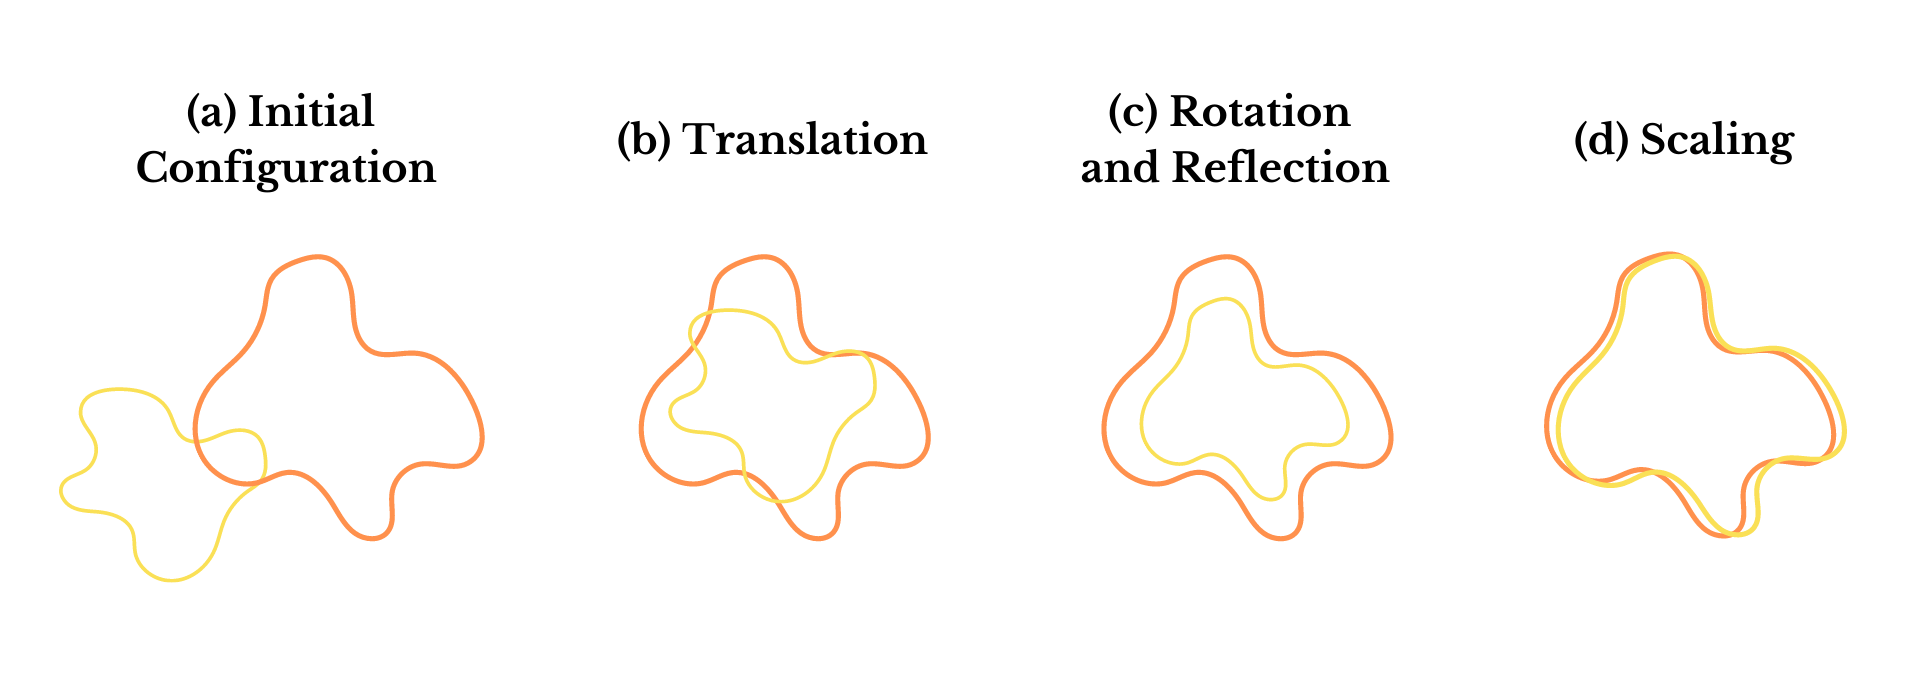
\includegraphics[width=1\linewidth]{sections/figures/orthogonal-procrustes.png}
  \caption{A general of example of the procrustes analysis where translation refers to the geometry transformation of moving every point of a space by the same amount of distance.}
  \label{fig:orthogonal-procrustes}
\end{figure}


On the other hand, the process of alignment is not always necessary for detecting LSC. The use of dynamic word embeddings helps alleviate the need for alignment. Temporal Referencing (TR), presented by \citet{dubossarsky-etal-2019-time}, is a method where diachronic corpora is treated as one corpus—sharing context information across time. This method was motivated by the fact that alignment should be circumvented as \citet{dubossarsky-etal-2017-outta} show that the process introduces noise. TR is a ``relabeling trick to achieve the same goals of the other dynamic methods while using a static embedding method" \citep{tahmasebi-survey2018}. Diachronic corpora are trained synchronically and vectors exist together in one vector space. Word vectors are situated in relation to each other and target words are relabelled and appended with a time-specific token (indicating which corpus they appear in) during training. Relabelling will only occur if the word is a target word. A word \emph{w} will not be relabelled and appear as a ``normal" word vector if it appears as a context word since this information can be shared across time periods. 